\documentclass[tikz,border=4pt]{standalone}
\usepackage{tikz}
\usetikzlibrary{arrows.meta,positioning,shapes.geometric,backgrounds,fit,calc}

\begin{document}
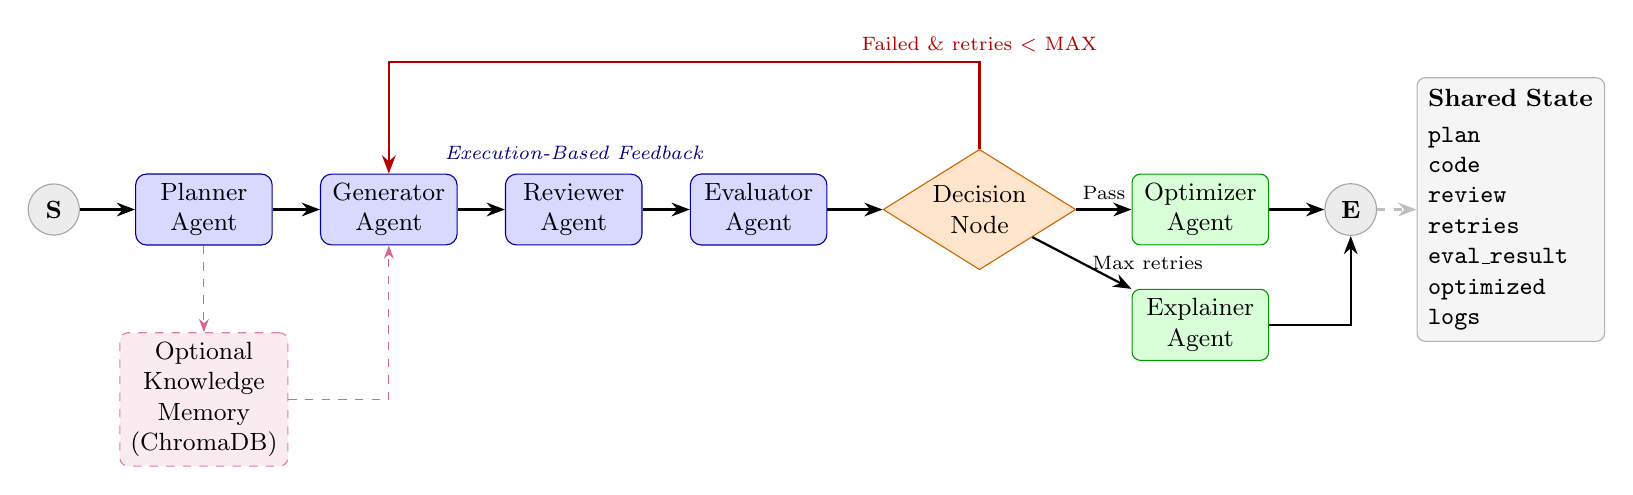
\begin{tikzpicture}[
  font=\small,
  >=Stealth,
  agent/.style={
    rectangle, rounded corners=4pt, draw=blue!60!black, fill=blue!15,
    minimum width=1.6cm, minimum height=0.8cm, text centered, text width=1.5cm
  },
  terminal/.style={
    circle, draw=gray!70, fill=gray!15,
    minimum size=0.65cm, font=\small\bfseries
  },
  decision/.style={
    diamond, draw=orange!80!black, fill=orange!20,
    minimum width=1.4cm, minimum height=1.0cm, aspect=1.6,
    text centered, text width=1.3cm, inner sep=1pt
  },
  outcome/.style={
    rectangle, rounded corners=3pt, draw=green!60!black, fill=green!15,
    minimum width=1.6cm, minimum height=0.8cm, text centered, text width=1.5cm
  },
  state/.style={
    rectangle, rounded corners=3pt, draw=gray!60, fill=gray!8,
    minimum width=2.2cm, text width=2.1cm, text centered
  },
  optional/.style={
    rectangle, rounded corners=3pt, draw=purple!50, fill=purple!8,
    minimum width=2.0cm, minimum height=0.8cm, text centered, text width=1.9cm,
    dashed
  },
  arr/.style={->, thick},
  redarr/.style={->, thick, draw=red!70!black},
]

%% Main pipeline nodes (horizontal)
\node[terminal]                        (start)  {S};
\node[agent, right=0.7cm of start]     (plan)   {Planner\\Agent};
\node[agent, right=0.6cm of plan]      (gen)    {Generator\\Agent};
\node[agent, right=0.6cm of gen]       (rev)    {Reviewer\\Agent};
\node[agent, right=0.6cm of rev]       (eval)   {Evaluator\\Agent};
\node[decision, right=0.7cm of eval]   (dec)    {Decision\\Node};
\node[outcome, right=0.7cm of dec]     (opt)    {Optimizer\\Agent};
\node[outcome, below=0.55cm of opt]    (exp)    {Explainer\\Agent};
\node[terminal, right=0.7cm of opt]    (end)    {E};

%% Optional RAG node (below pipeline)
\node[optional, below=1.1cm of plan]   (rag)    {Optional\\Knowledge\\Memory\\(ChromaDB)};

%% SharedGraphState (right side panel)
\node[state, right=0.5cm of end, align=left, inner sep=4pt] (state) {
  \textbf{Shared State}\\[2pt]
  \texttt{plan}\\
  \texttt{code}\\
  \texttt{review}\\
  \texttt{retries}\\
  \texttt{eval\_result}\\
  \texttt{optimized}\\
  \texttt{logs}
};

%% Main flow arrows
\draw[arr] (start) -- (plan);
\draw[arr] (plan)  -- (gen);
\draw[arr] (gen)   -- (rev);
\draw[arr] (rev)   -- (eval);
\draw[arr] (eval)  -- (dec);
\draw[arr] (dec)   -- node[above, font=\scriptsize]{Pass} (opt);
\draw[arr] (opt)   -- (end);
\draw[arr] (dec)   -- node[right, font=\scriptsize]{Max retries} (exp);
\draw[arr] (exp)   -| (end);

%% Retry arrow (red, looping back over pipeline)
\draw[redarr] (dec.north) -- ++(0,1.1)
  node[above, font=\scriptsize, text=red!70!black]{Failed \& retries $<$ MAX}
  -| (gen.north);

%% RAG query arrows (dashed)
\draw[->, dashed, purple!60] (plan.south) -- (rag.north);
\draw[->, dashed, purple!60] (rag.east)  -| (gen.south);

%% State panel connection
\draw[arr, gray!50, dashed] (end.east) -- (state.west);

%% Execution feedback label
\node[above=0.05cm of rev, font=\scriptsize\itshape, text=blue!50!black]
  {Execution-Based Feedback};

\end{tikzpicture}
\end{document}
